\section*{Introdução}
A artista brasileira Celeida Tostes (1929-1995) foi escultora, professora e uma das figuras centrais na expansão da cerâmica no Brasil, levando-a para além do campo utilitário e inserindo-a no horizonte da arte contemporânea. Sua performance \emph{Passagem} (1979) articula o fazer com o barro a experiências pessoais e coletivas, estabelecendo com a argila um vínculo visceral. Formada em instituições nacionais e internacionais, Celeida integrou a partir de 1975 o corpo docente da Escola de Artes Visuais (EAV) do Parque Lage, no Rio de Janeiro, e mais tarde da Universidade Federal do Rio de Janeiro, conciliando arte-educação e projetos comunitários em presídios e periferias.

Durante os anos de ditadura militar, o Parque Lage consolidou-se como polo de resistência e experimentação artística, reunindo artistas, críticos e estudantes em torno de uma pedagogia aberta e coletiva, em diálogo com a performance, a instalação e a escultura expandida. Nesse ambiente, a produção de Celeida, ao tratar de questões vividas por ela como mulher, aproximou-se das primeiras influências da segunda onda do feminismo no Brasil, articulando terra e gênero em rituais de renascimento e pertencimento.

É nesse horizonte que surge Passagem: coberta de argila líquida, a artista, com auxílio de suas assistentes, modela uma grande ânfora na qual adentra para depois emergir. A ação pode ser lida em dois registros complementares: no plano simbólico, próximo à leitura de Erich Neumann (1955/2015) e da arteterapia junguiana, que teve em Nise da Silveira uma pioneira, em que o vaso e a terra figuram como arquétipos do feminino; e no plano fenomenológico, herdeiro de Merleau-Ponty, que enfatiza a centralidade do corpo no mundo vivido.

O interesse da artista por Carl Gustav Jung e pelos conceitos arquetípicos do feminino reforça a pertinência de uma leitura que combine a escuta simbólica do barro com a experimentação artística do corpo em relação à matéria, herdeira da fenomenologia e do neoconcretismo. Ao mesmo tempo, a performance abre espaço para aproximações com a arteterapia, em que a co-criação com a matéria se torna ocasião para refletir sobre a subjetividade e convida à autorreflexão.

O objetivo deste artigo é refletir sobre a atualidade de Passagem, destacando sua linguagem simbólica do feminino e contrapondo-a à mercantilização da arte. Embora o recorte principal se concentre no período de 1975 a 1979, quando a performance foi realizada, é inevitável reconhecer que a obra projeta ressonâncias decisivas na década seguinte, funcionando como gesto-limiar: emerge sob a sombra da ditadura e dos experimentalismos dos anos 1970, mas já antecipa a abertura política e cultural dos anos 1980, quando práticas coletivas, pedagogias experimentais e articulações feministas ganharam novo fôlego no Brasil e na América Latina.

O texto organiza-se em três partes: (1) discute a importância do símbolo na psicologia analítica, na arteterapia, na fenomenologia e sua relação com o barro; (2) contextualiza a produção e a trajetória de Celeida no cenário político e artístico do Rio de Janeiro dos anos 1970; e (3) analisa a performance em articulação com as discussões anteriores e em relação ao conceito batailliano de \emph{informe}.

\begin{figure}[!t]
  \centering
  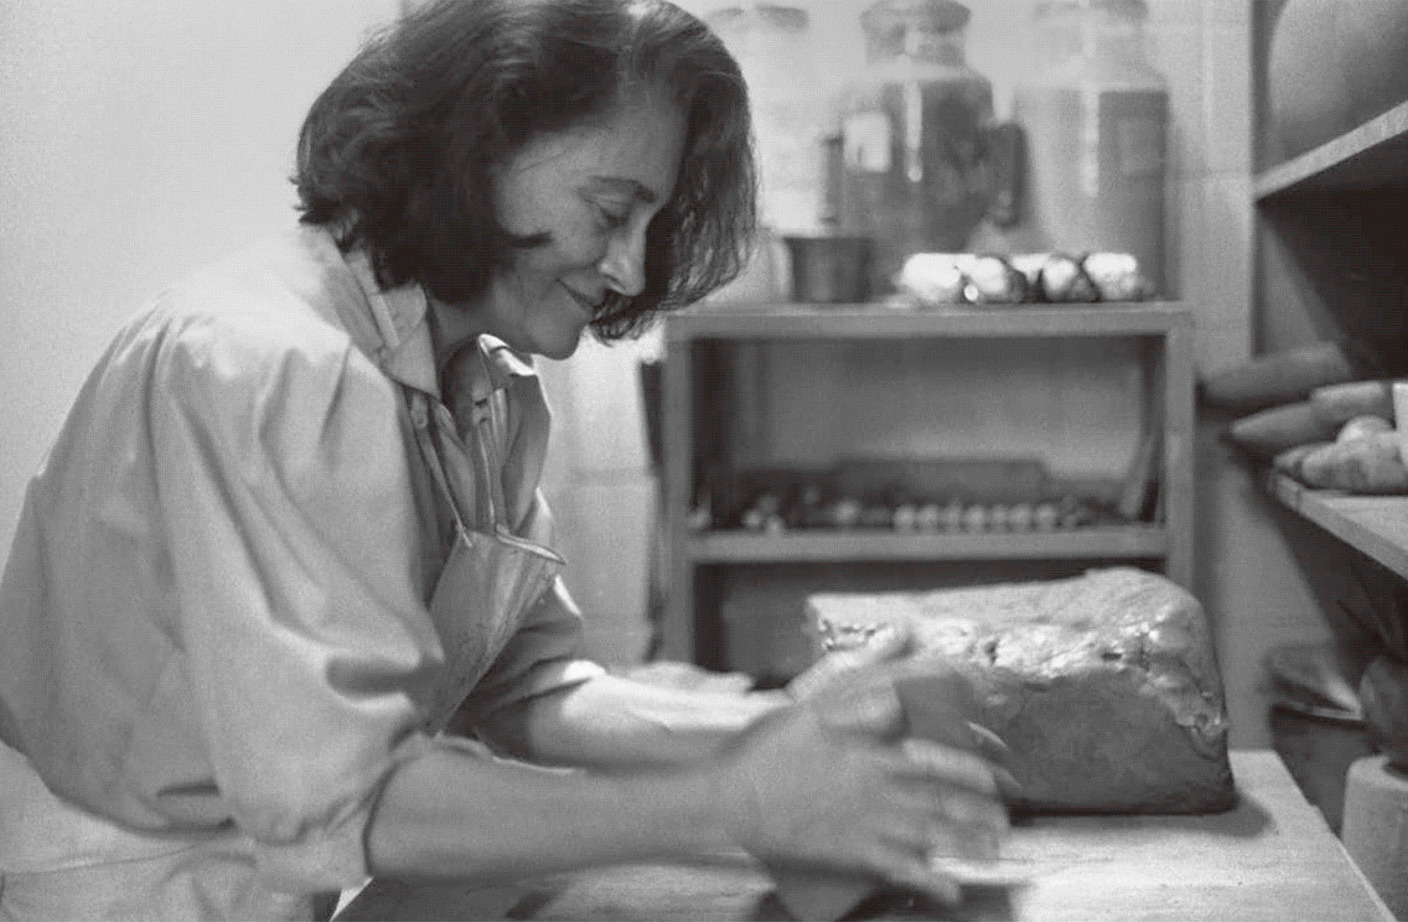
\includegraphics[width=0.8\linewidth]{figures/Celeida.jpg}
  \caption{Celeida Tostes. Fonte: Galeria Superfície. https://galeriasuperficie.com.br/artistas/celeida-tostes/.}
  \label{fig:celeida}
\end{figure}

\section*{O barro como símbolo e mito}
O barro, mais do que simples matéria-prima ou recurso utilitário ocupa um lugar singular na imaginação humana, presente desde os mitos de criação como matéria de origem, de transformação e de retorno. Não é apenas substância moldável, mas matriz criativa e campo de projeção arquetípica. A experiência simbólica que dele brota exige uma abordagem situada na subjetividade, dimensão essencial para a leitura de obras que o tomam como núcleo, como em Passagem. Embora resista a análises redutoras, a subjetividade foi explorada por diversas correntes filosóficas e psicológicas que reconheceram no símbolo uma linguagem própria do vivido \parencite{sassFlawGreatDiamond2022}.

Na modernidade, escritores como Proust e Valéry, assim como Cézanne nas artes visuais, transformaram a subjetividade em tema da criação, antecipando preocupações que seriam aprofundadas pela fenomenologia e pelo existencialismo. Esse movimento abriu caminho para que o símbolo fosse pensado como presença viva da subjetividade na experiência íntima do sujeito. Nesse mesmo horizonte, Goethe sintetizou a diferença entre alegoria e símbolo ao afirmar que “os símbolos são aquilo que representam” (apud Sass, 2022, p.25). O símbolo, assim, não aponta para além de si, mas participa da própria realidade que manifesta. Diferente do signo ou da alegoria, que remetem a significados fixos, o símbolo se abre ao indeterminado, transmitindo um sentido vivo e múltiplo.

A psicologia analítica acrescenta outra camada. Para Jung, o símbolo nunca esgota seu significado, apontando sempre além de qualquer conceito \parencite[p.60]{jacobiComplexoArquetipoSimbolo2021}. Edinger \citeyear{edingerEgoArchetypeIndividuation1992} enfatiza que ele oferece sentido à vida vivida, não em um significado fixo, mas como abertura para o desconhecido. Embora a teoria de Jung preserve um modelo estrutural do inconsciente, sua prática privilegia a escuta simbólica, aproximando-se, nesse ponto, da postura fenomenológica: reconhecer no símbolo um processo vivo, no qual interior e mundo se encontram na experiência do sujeito.

Essa visão amplia-se quando pensamos a criação não apenas como elaboração conceitual, mas como encontro físico com a matéria, em que o ato criativo, ao unir presença material e potência simbólica, torna-se campo privilegiado no diálogo entre subjetividade e símbolo. Essa abordagem é amplamente explorada na arteterapia junguiana, que no Brasil teve em Nise da Silveira sua principal pioneira. Ao reconhecer nas imagens produzidas por pacientes psiquiátricos símbolos vivos e não apenas sintomas, sua metodologia abriu caminho para uma prática terapêutica que valoriza a criação artística, a escuta sensível e a materialidade \parencite{silveiraImagensInconsciente2015}. Hoje difundida em ateliês, escolas e contextos terapêuticos, a arteterapia destaca-se por valorizar não apenas a interpretação de conteúdos inconscientes, mas também a experiência da co-criação entre sujeito e matéria. Como observa Urrutigaray (2023), nessa abordagem o símbolo não é um enigma a ser decifrado, mas uma presença que se manifesta no corpo, na matéria e no tempo da criação.

Gouvêa \citeyear{gouveaSolTerraUso2021}, ao citar Anaxágoras, “o homem pensa porque tem mãos” (p.68) acrescenta que o fazer manual não é a simples execução de uma ideia, mas pensamento que se dá no entrelaçamento de corpo, matéria e mundo. A mão imprime na matéria o que não pode ser elaborado em palavras; no contexto terapêutico, projeta conteúdos inconscientes em formas sensíveis. Criar com as mãos é, assim, mais do que produzir objetos: é instaurar uma linguagem em que a matéria se torna mediadora entre o subjetivo e o concreto.
Por sua resistência plástica ao tato e por instaurar uma temporalidade própria dentro da interação, a argila ocupa um lugar privilegiado. Modelar não se limita à obra final: abre um espaço simbólico em que imagens germinam e se transformam. Quando acompanhada por uma escuta simbólica, a prática com o barro revela dimensões que transcendem a sua materialidade. Nesse processo, emoções e imagens psíquicas pessoais se entrelaçam com conteúdos arquetípicos que encontram forma na manualidade. Cada ato individual de moldar a argila ativa, em escala íntima, narrativas coletivas e ancestrais. Essa matéria úmida e escura, tradicionalmente associada ao feminino, ao útero e à Lua, carrega um saber ancestral que convida à coautoria entre sujeito e mundo: “No barro, o homem cria e é criado” \parencite[p.73]{gouveaSolTerraUso2021}.

Não por acaso, mitos de diferentes tradições situam o barro como matéria primordial da criação. No antigo Egito, o deus Khnum era o oleiro divino que moldava os corpos humanos em seu torno, usando o lodo fértil do Nilo. Na tradição judaico-cristã, Adão, cujo nome deriva da palavra hebraica \emph{adamah} (terra), é formado do pó do solo e recebe o sopro divino como vida. A força desses mitos não reside apenas na narrativa, mas, segundo a psicologia analítica, na capacidade de ativar imagens do inconsciente coletivo, camada profunda da psique que abriga conteúdos transpessoais \parencite{jungOsArquetiposInconsciente2007}. Os arquétipos são as formas estruturais desse inconsciente: padrões universais de experiência que não possuem conteúdo fixo, mas se atualizam em imagens, mitos e símbolos sempre que encontram uma situação existencial correspondente na história de vida do sujeito. Os mitos, assim, são histórias coletivas que dão forma a essas potências, oferecendo imagens pelas quais o indivíduo pode elaborar conteúdos latentes.

Ainda nas narrativas que vinculam o barro à criação da humanidade destaca-se, na cosmologia iorubá, o mito de Nanã segundo o qual os corpos só puderam ser criados a partir da lama primordial, pois apenas essa matéria era capaz de acolher a vida. Trazido ao Brasil pela diáspora forçada da escravidão atlântica, esse mito se alojou no imaginário afro-brasileiro, tendo o barro como símbolo da ancestralidade, do feminino e da ligação entre origem e morte, entendida como retorno inevitável do ser humano à terra. Na psicologia analítica, essa dimensão é associada à Grande Mãe primeva \parencite{zacharias2025}, arquétipo que recebeu um estudo exaustivo de Erich Neumann, discípulo de Jung, ao desenvolvê-lo em \emph{A Grande Mãe} \citeyear{neumannGreatMotherAnalysis1955}.

Partindo do uroboros, símbolo da indiferenciação primordial, ele identifica na figura da Grande Mãe a primeira forma estruturante da psique coletiva, matriz a partir da qual se diferenciam tanto o masculino quanto outras manifestações do feminino. A partir dessa genealogia, Neumann percorre culturas, objetos rituais, esculturas e pinturas, identificando múltiplas expressões desse arquétipo. Sobre ela projetam-se aspectos ambivalentes: ora fonte de vida, cuidado e sabedoria, ora força destrutiva, possessiva e cruel. Essa polaridade não é um simples contraste, mas uma tensão constitutiva do feminino arquetípico. Neumann formula ainda a equação simbólica “mulher = corpo = vaso = mundo”, mostrando como esses elementos funcionam como recipientes equivalentes, espaços de germinação, abrigo e transformação.

Na criação de Celeida, vemos a reinterpretação poética dessa equação simbólica. O barro, enquanto matéria informe, remete à origem de toda criação; o vaso, ao ganhar forma, torna-se ventre de gestação e imagem do feminino como potência transformadora. É nessa atitude profundamente simbólica — entrar nua no recipiente, permanecer em seu interior e rompê-lo para renascer — que Celeida ressignifica o arquétipo no horizonte da arte de seu tempo.

\section*{Celeida e o Rio dos anos 1970}
Ao reinscrever a cerâmica no espaço da performance e da instalação, Celeida articula o cenário das artes de vanguarda do Rio de Janeiro dos anos 1970 com sua trajetória pessoal, marcada por viagens, leituras e pela experimentação constante com o barro. A argila torna-se uma amálgama que media dimensões simbólicas e concretas, individuais e coletivas, psicológicas e artísticas, ligando a criação da artista ao tecido social de seu tempo.

\begin{figure}[!t]
  \centering
  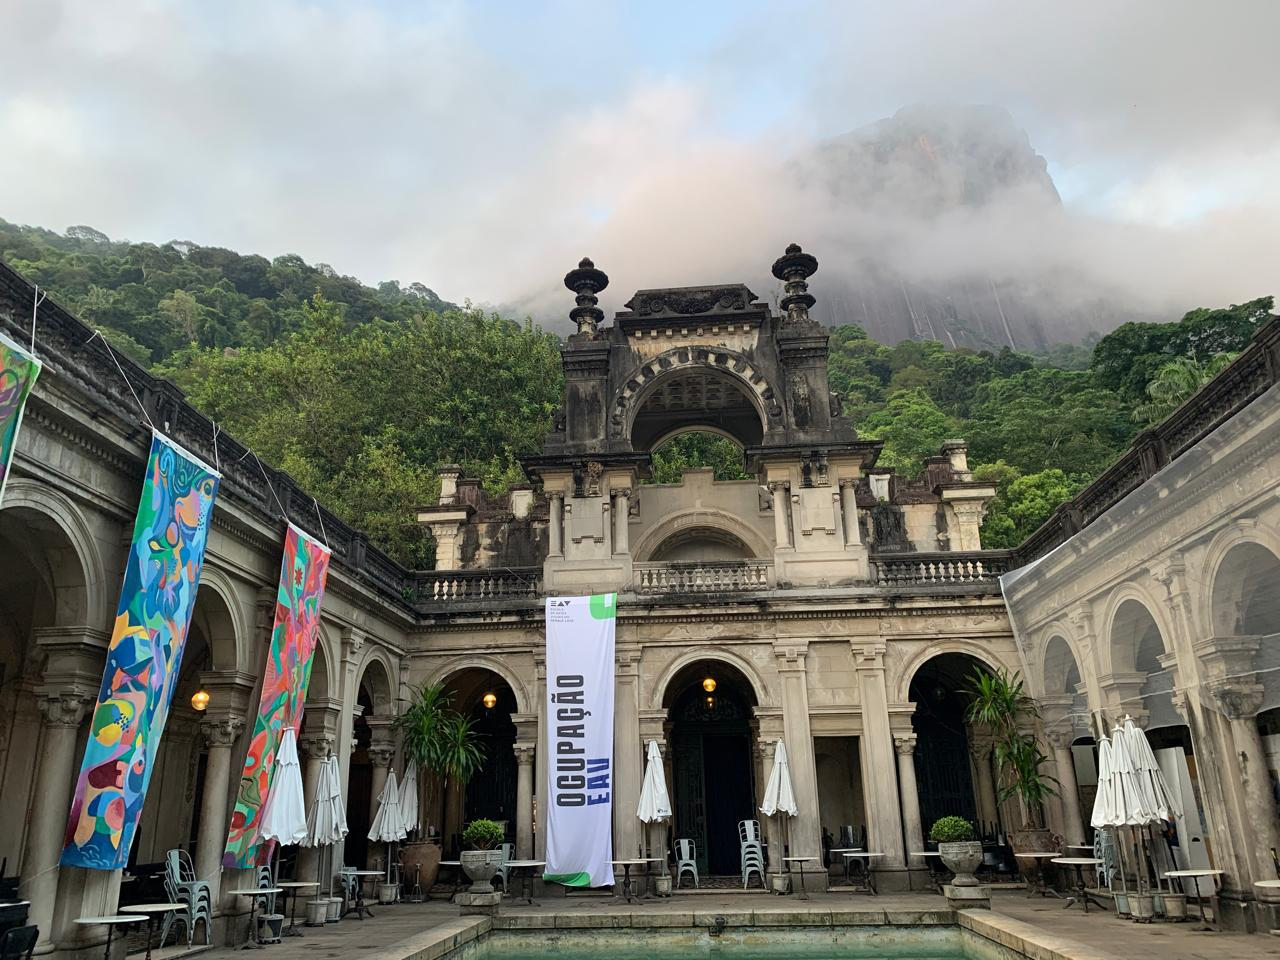
\includegraphics[width=0.8\linewidth]{figures/parque_lage.jpg}
  \caption{Escola de Artes Visuais do Parque Lage. Fonte: Foto do autor.}
  \label{fig:parque-lage}
\end{figure}

Seu trabalho dialoga com debates críticos da época, que defendiam uma arte experimental e aberta em contraposição aos modelos tradicionais e hierárquicos de representação e apreciação. Nesse horizonte, aproximava-se das proposições de Frederico Morais — como nos eventos do Museu de Arte Moderna do Rio, \emph{Domingos de Criação} (1970), e da mostra \emph{Do Corpo à Terra} (1971), no Parque Municipal de Belo Horizonte —, assim como das heranças do neoconcretismo e do espírito híbrido da tropicália.

Essa postura da vanguarda artística contrastava com o contexto brasileiro da ditadura militar. Nos anos 1970, o país atravessava a transição entre o auge da repressão política e do crescimento econômico para, já na segunda metade da década, sob o governo do general Ernesto Geisel, mergulhar em crise econômica e iniciar a chamada “distensão”, projeto dos militares por uma abertura lenta e controlada rumo ao governo civil.

Nesse mesmo período, a segunda onda do feminismo (1960-1980) ampliava a luta das mulheres para além dos direitos civis e políticos, trazendo à tona pautas como liberdade sexual, direito ao aborto e crítica ao patriarcado, sob o lema “o pessoal é político” (Marques; Xavier, 2018). No Brasil, entretanto, a assimilação foi tardia e atravessada pela censura da ditadura e pela circulação restrita de obras teóricas, sendo mediada por autoras como Heloneida Studart, Rose Marie Muraro e Carmen da Silva, cuja coluna na revista \emph{Cláudia} difundiu ideias feministas adaptadas ao cotidiano. O estigma da feminista como “violenta” ou “destruidora de lares” levou muitas artistas a evitarem vínculos explícitos com o movimento, embora textos de Carmen da Silva tenham influenciado nomes como Anna Maria Maiolino, Wanda Pimentel, Iole de Freitas e Letícia Parente, que problematizaram corpo, vida doméstica e estereótipos de gênero em plena ditadura \parencite{trizoliCriticaArteFeminismo2012}.

Foi nesse cenário, marcado por diferentes vertentes feministas, pela produção artística das mulheres e pelo ambiente repressivo da ditadura, que Celeida retornou ao Rio de Janeiro em 1975. Convidada a lecionar na recém-inaugurada Escola de Artes Visuais do Parque Lage, encontrou ali um espaço que rapidamente se consolidaria como um dos núcleos mais férteis de resistência cultural e de reinvenção do ensino da arte no Brasil.

Localizada em uma antiga mansão cercada por jardins e pela mata atlântica, a EAV tornou-se um dos principais polos de liberdade criativa durante a ditadura militar. A transferência da Escola de Belas Artes e de outros cursos da Universidade Federal do Rio de Janeiro para o campus isolado da Ilha do Fundão contribuiu para esse papel: em contraste com o afastamento, o Parque Lage emergiu como um dos poucos espaços urbanos abertos, que articulava em seus programas de ensino uma prática crítica e experimental. Diferente do modelo acadêmico tradicional, estruturava-se como um ambiente horizontal e coletivo, em que professores e alunos compartilhavam oficinas, debates e práticas artísticas interdisciplinares. Sua pedagogia não se restringia ao domínio técnico, mas dialogava com modelos como a Black Mountain College, sempre reinterpretados à luz da realidade brasileira e de experiências de criação artística fora da academia.

Nesse campo didático inovador, lembra Saldanha \citeyear{saldanhaEscolaArtesVisuais2017}, a escola dialogava com a experiência pioneira de Nise da Silveira, que nos anos 1950 criou o Museu de Imagens do Inconsciente, transformando a clínica psiquiátrica em espaço de produção simbólica e de escuta do inconsciente coletivo. Sua prática ofereceu uma alternativa ao autoritarismo médico e abriu novos ambientes para a criação artística fora da academia. Além disso, a defesa de uma educação integrada pela arte proposta por Herbert Read e a pedagogia libertadora de Paulo Freire, formulada nos anos 1960, fortaleceram o horizonte teórico-prático da escola.

Nesse contexto, a presença de Celeida Tostes foi decisiva para consolidar um espaço sensível às questões da vanguarda. Como recorda Hélio Eichbauer, “a Celeida, com o barro, com a argila, recriou um mundo. Havia uma questão ancestral, o ritual da criação. Isso se tratava muito no começo da escola” \parencite[p.277]{saldanhaEscolaArtesVisuais2017}. Sua prática, retomando imagens arquetípicas como o “ovo cósmico”, inscrevia-se em diálogo com a psicologia junguiana, ao articular o barro a expressões do inconsciente coletivo.

\begin{figure}[!t]
  \centering
  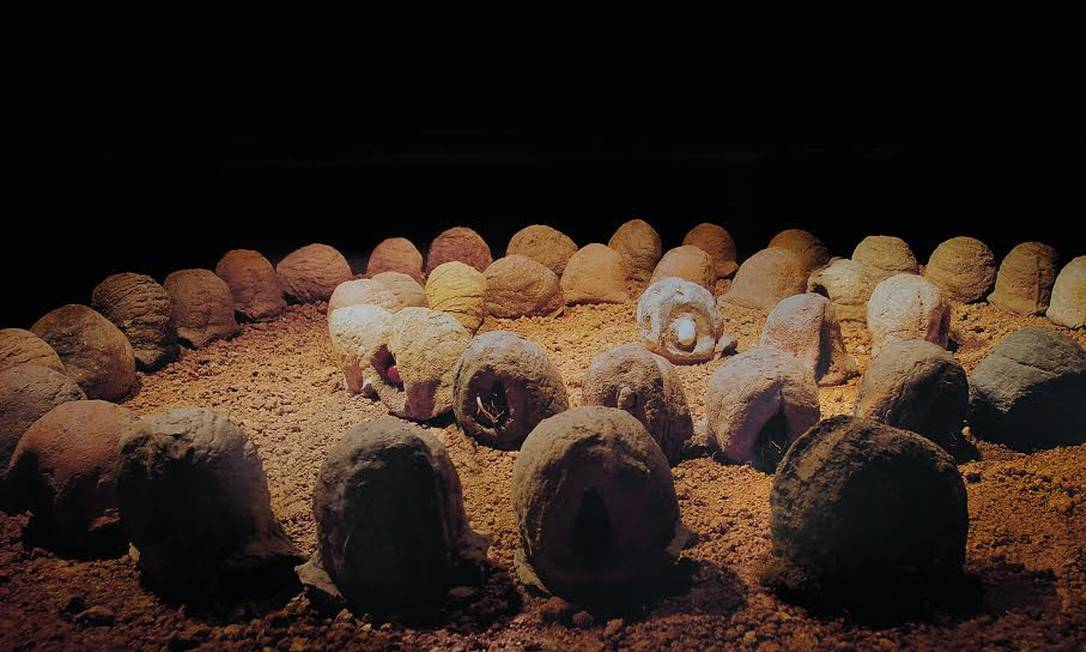
\includegraphics[width=0.8\linewidth]{figures/aldeia_furnarius_rufus.jpg}
  \caption{\emph{Aldeia Furnarius rufus}. Instalação exibida na I Bienal do Barro da América, Caracas, 1992. Foto: Divulgação / Acervo Suzete Muzeraqui.}
  \label{fig:furnarius}
\end{figure}

Suas oficinas, baseadas no contato direto com a matéria e na experimentação sensorial, desestabilizavam hierarquias e abriam espaço para processos criativos inesperados. Dessa experiência nasceu o neologismo criado pelo colega e pintor Luiz Áquila: \emph{celeidar}, verbo que sintetizava sua potência pedagógica — mais que ensinar técnicas, tratava-se de provocar deslocamentos e abrir caminhos de criação coletiva. Sua sala de aula funcionava como um ateliê compartilhado, em que processo e escuta ocupavam posição central. Criar obras de arte significava também transformar a si mesmos — inclusive Celeida, enquanto mediadora desse processo.

A prova disso é que, no mesmo ano em que realizou Passagem, ela ampliou seu projeto pedagógico-artístico ao iniciar sua atuação na comunidade do Chapéu Mangueira, no Leme, implantando um núcleo de cerâmica utilitária junto às mulheres da favela. O trabalho refletia o mesmo princípio vivido no Parque Lage: um aprendizado em via de mão dupla. O barro, que para a artista representava reconexão com suas próprias origens, tornava-se também mediador de identidade cultural e de sustento para os moradores. Foi nesse ambiente colaborativo que sua prática se consolidou em obras emblemáticas, reafirmando a dimensão comunitária e não autoral.

Em \emph{Aldeia Furnarius rufus} (fig.\ref{fig:furnarius}), inspirada no joão-de-barro, ela recriou dezenas de casas em espiral e convidou crianças e grupos diversos a construir uma “cidade ideal”, dissolvendo a autoria individual em processo compartilhado. Já em \emph{O Muro} (1982), uma imensa construção de adobe erguida em mutirão por artistas, alunos e moradores do Chapéu Mangueira, a autoria se dispersou em ação coletiva, e a obra transformou-se em símbolo ambivalente de separação e encontro (Silva, 2006).

Esse modo de atuar dialogava com o clima político dos anos 1980. Como observa Daniela Name \citeyear{nameLamaAoCaos2014}, após décadas de polarização entre capitalismo e socialismo e da repressão da ditadura, a militância se deslocava da praça pública para esferas íntimas e comunitárias. A política passava a ser exercida no cotidiano, nos coletivos artísticos e nas redes de afetos. É nesse contexto que a docência de Celeida se insere, convertendo a sala de aula em ateliê partilhado e projetando esse espaço para a rua e a comunidade, em um movimento de criação coletiva, pensamento crítico e liberdade — atitudes que, em pleno regime autoritário, soavam subversivas.

Essa fusão entre criação e vida, intensificada a partir do final dos anos 1970, reencontra uma linhagem aberta décadas antes pelo neoconcretismo. Desde o final dos anos 1950, artistas como Lygia Clark, Lygia Pape e Hélio Oiticica propuseram uma arte que deixava de ser objeto autônomo para tornar-se experiência sensível, definida como “não-objeto” por Ferreira Gullar e como “proposição” por Oiticica. O corpo e a participação tornaram-se centrais, e a figura do artista deslocou-se da posição de “gênio criador” para a de propositor ou educador \parencite{caysesIstoNaoUma2014}. Essa afinidade manifesta-se também na valorização do processo, da experiência fenomenológica e da presença no espaço vivido, em consonância com a filosofia de Merleau-Ponty \parencite{gullarManifestoNeoconcreto1959}. Assim como os neoconcretos buscaram romper com o formalismo construtivo para aproximar arte e vida, Celeida enfatizou o processo, o corpo e a partilha como núcleos de criação.

Sob esse enfoque, a artista revela afinidades diretas com os experimentos de Lygia Pape e Lygia Clark. Como observa Name \citeyear{nameLamaAoCaos2014}, “há uma ligação bastante potente entre Passagem e as experiências Ovo, de Lygia Pape, e A casa é o corpo, de Lygia Clark” (p.58). Em todos esses casos, o corpo atravessa um espaço simbólico, transformando a estética em acontecimento e colocando em crise a noção de obra de arte como mercadoria. Nesse sentido, a performance partilha da subversão presente nas proposições de Clark e Pape e se afirma como gesto político e anticapitalista, ao mesmo tempo em que testemunha uma dimensão feminina do fazer.

\section*{A obra \emph{Passagem} (1979)}
A performance, realizada em sua casa em Botafogo e registrada por Henry Stahl, contou com a ajuda de duas assistentes. Com elas, Celeida ergueu pelo método do acordelado uma grande ânfora de barro, na qual se colocou nua, depois de cobrir o corpo com argila líquida. A peça foi então selada e, após permanecer algum tempo em seu interior, a artista rompeu as paredes e deslizou para fora. Em relatos posteriores, Celeida afirmou ter sido transformada pela experiência, inaugurando um período de aprofundamento em sua relação com a argila.

\begin{figure}[!t]
  \centering
  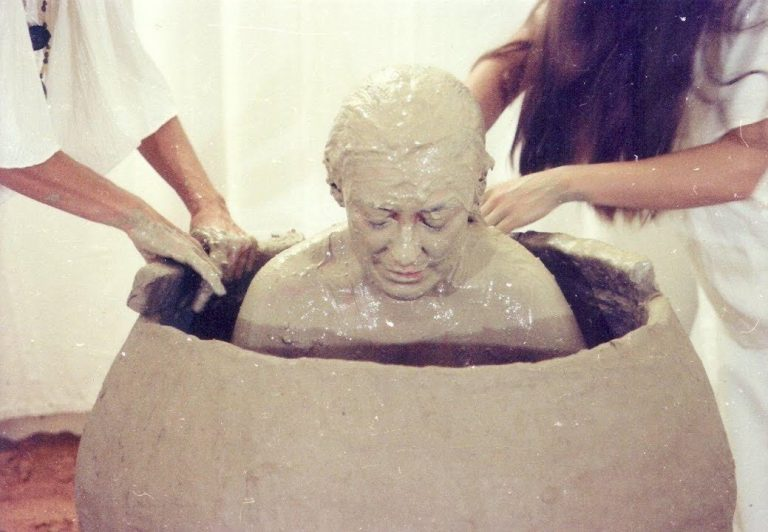
\includegraphics[width=0.8\linewidth]{figures/passagem_1.png}
  \caption{Escola de Artes Visuais do Parque Lage. Fonte: Foto do autor.}
  \label{fig:passagem-1}
\end{figure}

A ampliação do vaso à escala humana serve como metáfora da expansão do potencial terapêutico para a esfera da arte contemporânea. Aqui se evidencia uma dinâmica próxima à arteterapia de Nise da Silveira, em que a matéria, em contato com o corpo, atua como veículo de elaboração psíquica. Isso também se conecta a leituras simbólicas tradicionais, nas quais o ato de moldar o vaso associa-se ao feminino e à maternidade. Além disso, sua declaração após a performance — “tive contato com alguma coisa que era como um útero […] Eu acho que trepei com o barro” \parencite[p.225]{SilvaBiografia2014} — pode ser lido como uma experiência urobórica descrita na qual a consciência se dissolve na indiferenciação primordial e todos os opostos se confundem no arquétipo da Grande Mãe. O vaso torna-se, assim, não apenas cápsula de travessia, mas também espaço de fusão erótica, extática, atualização corporal de um estado psíquico em que corpo e mundo ainda não se separam. Em contraste, o masculino aparece apenas como guardião da imagem: Henri Stahl fotografa, e seu testemunho silencioso do olhar masculino apenas entrevê o aspecto misterioso da experiência, acentuando a centralidade feminina da obra.

É nesse entrelaçamento de presenças, afetos e interpretações que o símbolo revela sua vitalidade: não como imagem fixa, mas como forma em processo, que não substitui um conteúdo já dado, mas aponta para o que pode surgir de sua potência. Seu papel é prospectivo: suscitar sentidos, reativar o processo de conhecimento e abrir caminhos para a subjetividade. Assim, o mais fecundo nesta intervenção não é decidir se o vaso é útero, túmulo ou travessia, mas aceitar que é tudo isso ao mesmo tempo — e ainda outra coisa para cada olhar. Símbolos são como vasos comunicantes: não encerram uma equivalência rígida, mas permitem que os sentidos se transfiram e se renovem.

Somado a isso, Passagem adquire também uma dimensão política do feminino: em plena ditadura, quando o corpo era alvo de censura e controle, Celeida reivindica a nudez não como motivo erótico, mas como sujeito criador. Ao se colocar nua dentro de um vaso de barro, confronta o moralismo patriarcal da época e situa o corpo feminino como matriz simbólica e produtiva, em diálogo com as críticas feministas que circulavam no ambiente artístico latino-americano. Se o feminismo — assim como a arte — buscava ampliar seu alcance para abarcar questões do cotidiano e da intimidade, Celeida traduz esse movimento para a linguagem do barro, onde o íntimo se torna público e o simbólico se faz coletivo. Sua obra não replica discursos estrangeiros: emerge da realidade brasileira, evocando tanto as urnas funerárias indígenas quanto os rituais afro-brasileiros ligados à terra, e articula barro, corpo feminino e pedagogia em uma poética que atualiza o feminino arquetípico.

Décadas depois, autores estrangeiros como Suzi Gablik e Michel Maffesoli ofereceram chaves para compreender tensões entre espiritualidade, coletividade e essencialismos que também atravessam a recepção da obra de mulheres artistas. Gablik, em \emph{The Reenchantment of Art} (1991), defendeu uma arte espiritual, comunitária e ecológica, próxima de certas vertentes ecofeministas, mas criticada por reproduzir dualismos como natureza/feminino versus cultura/masculino. Já Maffesoli propôs um “reencantamento do mundo” baseado em identidades plurais e relacionais, enraizadas em mitos, imaginários e formas de sociabilidade afetiva \parencite{trizoliTrajetoriasReginaVater2011}. Essa camada está presente no trabalho de Celeida: embora exista uma identificação do vaso como útero, na sua intervenção emerge também a imagem de um corpo coletivo da terra, lugar de comunhão com a origem, com o feminino arquetípico e com a memória primeira dos seres vivos. A artista nos lembra de uma força subterrânea que pulsa em cada nascimento, em cada ato de cuidado e no retorno à terra.

Para compreender o aspecto processual da obra, é preciso atentar também para a técnica ancestral do acordelado, transmitida por mulheres indígenas e utilizada na moldagem do vaso \parencite{dutraPalcoAoBarro2022}. O processo repetitivo, lento e fisicamente exigente envolve todo o corpo e conduz a um estado de imersão sensível, em que o sentido da obra não se fixa em um projeto prévio, mas emerge da experiência vivida. Essa dimensão também atravessava sua prática pedagógica: como lembra Ricardo Ventura, ex-aluno da Oficina da EAV das Artes do Fogo, parte do método de Celeida consistia justamente em forçar o desapego da ideia de “obra pronta”. Ele recorda que, ao vê-lo contemplar satisfeito uma peça que acabara de concluir, Celeida a derrubou no chão, reduzindo-a a cacos. O gesto, que num primeiro momento provocou raiva, revelou depois sua lição: o essencial não era o objeto acabado, mas o processo, o caminho, a transformação que o fazer instaurava \parencite[p.56]{nameLamaAoCaos2014}.

É nesse mesmo horizonte que a performance pode ser lida à luz da noção de quasi-corpus, desenvolvida por Lygia Clark no âmbito do neoconcretismo. Para Clark, o quasi-corpus designa uma categoria liminar entre obra e corpo: o objeto artístico deixa de ser autônomo e passa a existir apenas no acontecimento da experiência. Nem corpo biológico, nem escultura autossuficiente, trata-se de uma entidade híbrida, ativada pela interação. Nesta atitude, Celeida radicaliza o princípio: o vaso de barro não é simples recipiente, mas um corpo-outro que envolve, contém e é rompido pelo corpo da artista. A fusão entre corpo e matéria, mediada pela técnica do acordelado, cria um espaço fenomenológico em que sujeito e objeto se confundem.

Finalmente, vale recorrer às próprias palavras de Celeida, escritas logo após a ação, para perceber como sua criação não se apresentava como objeto acabado, mas como experiência de dissolução e recomposição de limites — inclusive formais:

\begin{citacao}
  Despojei-me\\
  Cobri meu corpo de barro e fui.\\
  Entrei no bojo do escuro, ventre da terra.\\
  O tempo perdeu o sentido de tempo.\\
  Cheguei ao amorfo.\\
  Posso ter sido mineral, animal, vegetal.\\
  Não sei o que fui.\\
  Não sei onde estava. Espaço.\\
  A história não existia mais.\\
  Sons ressoavam. Saíam de mim.\\
  Dor.\\
  Não sei por onde andei.\\
  O escuro, os sons, a dor, se confundiam.\\
  Transmutação.\\
  O espaço encolheu.\\
  Saí. Voltei.\\
  (Celeida Tostes apud Dutra, 2022, p.15)
\end{citacao}

Esse testemunho acentua o caráter processual da obra: não a fixação de uma forma, mas o mergulho no amorfo, naquilo que se transforma incessantemente. É a partir dessa dimensão que podemos compreender Passagem também sob a chave do termo informe, criado por Georges Bataille (1897-1962). Lançado nos anos 1920 como verbete do Dictionnaire critique, o informe não designa um conceito fixo, mas um gesto de “trazer as coisas para baixo”, desmontando categorias elevadas e recusando significados estáveis. Revisitado por Krauss e Bois \citeyear{boisFormlessUsersGuide1997}, na exposição \emph{L’informe: mode d’emploi}, o termo foi mobilizado para expor fissuras do próprio modernismo, mostrando como a arte já continha forças capazes de desestabilizar a oposição entre formalismo e iconologia.

No campo artístico, o informe não é simples ausência de forma, mas aquilo que perturba hierarquias entre forma e matéria, liberando resíduos, manchas, restos e processos inacabados como operadores estéticos. Contra a promessa modernista de uma essência autônoma da arte, propõe uma abertura crítica em que a matéria resiste a qualquer desenho prévio.

Nesse sentido, Passagem pode ser lida como profundamente informe. O barro, material comum e alheio ao circuito nobre das belas artes, torna-se operador de desestabilização, recusando a idealização formal e deslocando a criação para o terreno da experiência. Em plena ditadura, quando a linguagem modernista era em parte assimilada como projeto oficial de Estado, a obra afirma o barro como força de resistência: prática em que subjetividade, corpo e matéria se tornam indissociáveis e críticas à ordem estabelecida.

\begin{figure}[h]
  \centering
  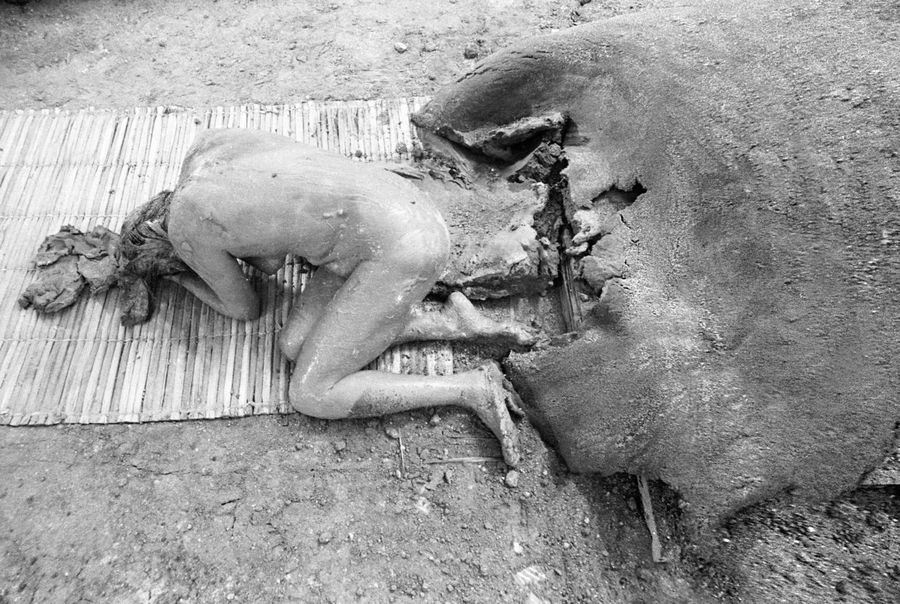
\includegraphics[width=0.8\linewidth]{figures/passagem_2.jpg}
  \caption{Escola de Artes Visuais do Parque Lage. Fonte: Foto do autor.}
  \label{fig:passagem-2}
\end{figure}

\section*{Conclusão}
Essa obra condensa as tensões políticas e possibilidades poéticas que atravessavam o Brasil dos anos 1970: a ditadura militar, as primeiras articulações feministas e o diálogo com a herança neoconcreta. Enquanto o neoconcretismo dissolvia as fronteiras entre arte e vida pela via da percepção e da experiência fenomenológica, Celeida acrescenta uma dimensão espiritual e simbólica que torna Passagem singular. Nos anos 1970, introduziu o barro no circuito artístico brasileiro como mediador de identidades, memórias e coletividades — prática que se expandiria em obras como \emph{Aldeia Furnarius rufus} e \emph{O Muro}.

Em \emph{Passagem}, vida, barro e criação se confundem. Ao entrar em um vaso de argila e deixar-se envolver pela terra, a artista assume uma postura corajosa de entrega, próxima aos mitos de katábasis, a descida ritual ao interior da terra e ao inconsciente. A leitura de Neumann \citeyear{neumannFearFeminineOther1994}, esclarece o alcance dessa entrega: ser filho ou filha da terra implica reconhecer nossa condição frágil e compartilhada. A performance encarna essa atitude ao abdicar do controle formal, deixar-se imprimir pela matéria e aceitar o peso da terra sobre o corpo e nossas estórias. 

Esse gesto pode ser lido também como reação ao projeto modernista da arte e ao patriarcado, que exigiam papéis a cumprir e formas a alcançar. Em lugar disso, Celeida reabre a experiência estética como encontro improvisado entre corpo e mundo, afirmando o barro como espaço de reconciliação: coragem de ser mulher, artista e educadora nos anos 1970, acolhendo ao mesmo tempo a potência da escuta e da transformação.

Como lembra Rilke, somos “abelhas do invisível” quando transmutamos o efêmero em substância espiritual, fazendo do vivido uma forma que permanece em nossa subjetividade. Preservar a terra, nesse horizonte, não é apenas ação exterior, mas condição para que a alma humana se constitua e se nutra. É nesse movimento, quando a terra se converte em presença íntima, que as palavras de Rilke se abrem para novas possibilidades, como no vaso de Celeida:

\begin{citacao}
  A terra não tem outra saída senão tornar-se invisível: em nós, que com uma parte de nossa natureza participamos do invisível, temos (ao menos) parte nele, e podemos aumentar nossas reservas do invisível durante nossa estada aqui — somente em nós pode consumar-se essa íntima e duradoura conversão do visível em um invisível que já não depende de ser visto e tocado, assim como nosso próprio destino cresce continuamente, ao mesmo tempo MAIS PRESENTE E INVISÍVEL em nós. \parencite[p.445]{rilkeLetterWitoldHulewicz1972}
\end{citacao}

A importância desta obra, enfim, não se limita ao gesto que a originou. Ela nos convida a pensar a crítica de arte a partir de uma escuta simbólica: não reduzir a criação ao seu conteúdo imediato, mas reconhecê-la como processo vivo, capaz de reativar sentidos latentes e instaurar novas relações entre corpo, matéria e subjetividade. Assim, a crítica deixa de ser apenas interpretação ou juízo para tornar-se também espaço de abertura — lugar em que a arte continua a falar e a suscitar respostas em diferentes contextos.
